\documentclass{article}
\usepackage{amsmath}
\usepackage{fancyhdr}
\usepackage{amsmath}
\usepackage{clrscode}
\usepackage{subfigure}
\usepackage[top=3cm, bottom=3cm, left=3cm, right=3cm]{geometry}
\usepackage[pdftex]{graphicx}\title{BME511L: Literature Search Report}
\usepackage{float}
\usepackage{amsfonts}
\author{Allen Yin}
\pagestyle{fancy}
\setlength\parindent{0.0in}
\setlength\parskip{0.0in}
\usepackage{caption}
\captionsetup{justification=justified}
\setcounter{tocdepth}{2}
\setlength{\headheight}{15pt}

\begin{document}
\maketitle
\setlength\parskip{0.1in}

The brain consists of about $10^{10}$ neurons, with varying shape, size, and orientations. Invidivudal neurons can generate a small amount of electrical activity, which cannot be picked up by surface electrodes on the scalp. However, when a large group of neurons is simultaneously activated, the resulting electrical activity is large enough to be picked up by the electrodes at the surface, generating the Electroencephalography (EEG).

\section{Literature Search}
EEG has been measured as a clinical signal since the 1930s. The information extracted from these signals was first used in the diagnoses of neurological diseases, mainly epilepsy. Most older EEG modeling literature (prior to early 2000's) used idealized concentric spherical shell models first used in the EKG literature \cite{EKG}, resulting in many analytical results. In addition, many modeling papers have been focused on more efficient computational methods in the context of these idealized models. As computational power become more available, EEG modeling became more realistic and computational. The computational models have since used 3D, realistic headshapes, conductivities and anisotropy.

The current focus of EEG research is focused on source localization. It consists of solving a forward and inverse problem. Solving the forward problem starts from a given electrical source configuration representing neurons in the head, then the potentials at the electrodes are calculated for this configuration. The inverse problem attempts to find the electrical source which genreated a measured EEG. By solving the inverse problem, repeated solutions of the forward problem for different source configurations are thus needed \cite{HanzReview}. The goal of source localization is to apply the technique to find correlations between measured EEG and theunderlying neural mechanisms.

\section{Candidate Papers}
Literature search in EEG modeling seems to suggest there isn't a very smooth transition in terms of complexity from the older analytical concentric spherical shell models \cite{Schneider}\cite{Fender} to the modern, computationally intensive realistic EEG-head models.

The paper I will base my modeling on is Yan, Nunez, and Hart's 1991 paper \emph{Finite-element model of the human head: scalp potentials due to dipole sources}\cite{Yan}. In this paper, the source of EEG is modeled by dipole sources within different shaped head models. First, concentric spherical shells with different conductivities (brain, skull, and scalp) head model was first used to serve as a sanity check, and to establish the grid density for FEM. Then a more realistic head model was constructed by manual geometric measurements of a skull. FEM was then ran on this realistic model with different dipole source locations to compare the difference of the results between the realitic and ideal head model.

The geometry of the used head models are shown in the figures below.

\begin{figure}[H]
    \begin{center}
        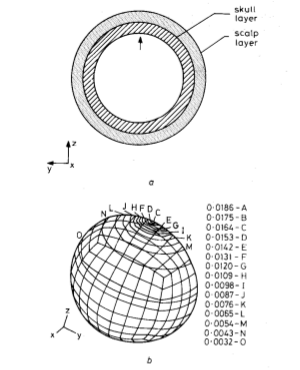
\includegraphics[scale=0.6]{sphere.png}
        \caption{Spherical head model gemoetry\cite{Yan}}
    \end{center}
\end{figure}

\begin{figure}[H]
    \begin{center}
        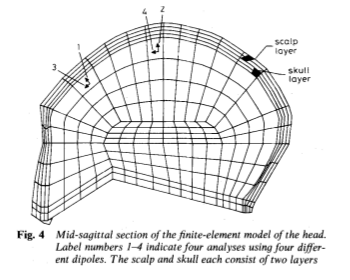
\includegraphics[scale=0.6]{head.png}
        \caption{Realistic head model geometry - mid-sagittal section \cite{Yan}}
    \end{center}
\end{figure}

\begin{figure}[H]
    \begin{center}
        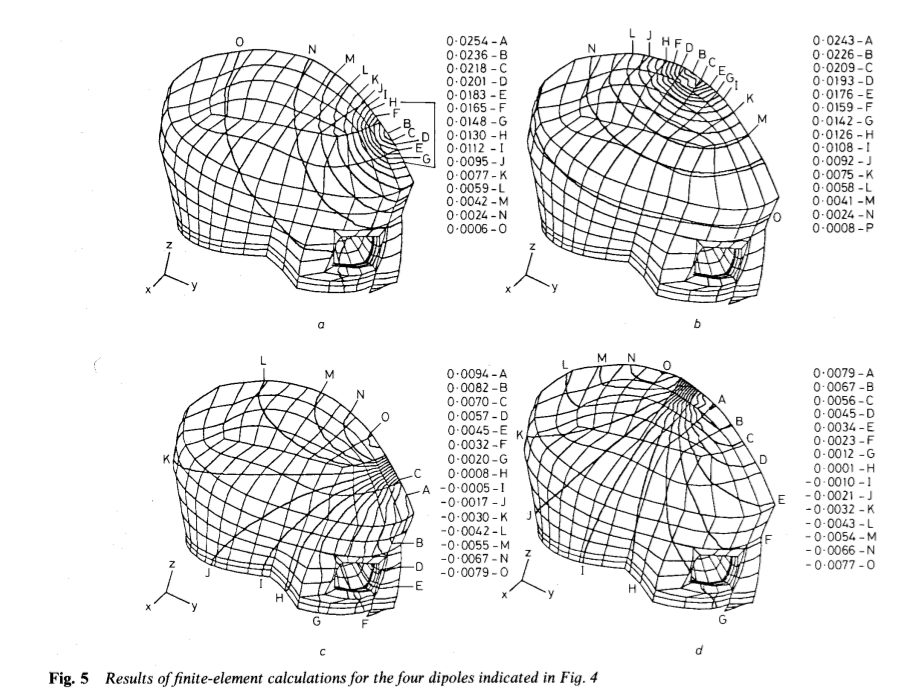
\includegraphics[scale=0.5]{headall.png}
        \caption{Realistic head model geometry and equipotential lines \cite{Yan}}
    \end{center}
\end{figure}

\section{Modifications}
Ideally, I would like to perform modeling on a realistic 3D head shape, obtaining parameters either through literature search or manual measurements of a skull model. I would follow Yan's approach of dividing the realistic headshape into three concentric shells with homogeneous conductivity to keep the computational complexity down. I would then introduce dipole sources at different locations and calculate the potential and current densities with flexPDE. I can also introduce electrode pair locations on the head and model their effects on the EEG potentials.

One possible complication is that, as Yan points out in his paper, the 3D spherical model required 6402 nodes, the realistic head model required 8487 nodes using his custom FEM algorithms. Since flexPDE student edition has a 3D node-limit of 1600, I might not be able to achieve exactly what I planned. If that's the case, several additional modifications can be tried:
\begin{itemize}
    \item Decrease the boundary complexity of the realistic head model, forming the boundaries with smoother segments.
    \item Split the head on the sagittal plane to reduce the complexity by half.
    \item Model the head in sections - Only the frontal, parietal, or occipital lobe sections are modeled at a time. However, this would limit the combination of electrode and source placements.
    \item Model a mid-sagittal plane 2D realistic head, or a quarter spherical model.
\end{itemize}

\begin{thebibliography}{3}
        \bibitem{EKG}
            Arthur, R.Martin; Geselowitz, David B., ``Effect of inhomogeneities on the apparent location and magnitude of a cardiac current dipole source'', \emph{Biomedical Engineering, IEE Transactions on}, April 1970.
        \bibitem{HanzReview}
            Hallez, Hans et al. ``Review on Solving the Forward Problem in EEG Source Analysis'', \emph{Journal of NeuroEngineering and Rehabilitation}, 2007.
        \bibitem{Yan}
            Yan, Y; Nunez, P.L.; Hart, R.T., ``Finite-element model of the human head: scalp potentials due to dipole sources'', \emph{Medical and Biological Engineering and Computing}, September 1991.
        \bibitem{Schneider}
            Schneider, Michel; ``Effect of inhomogeneities on surface signals coming from a cerebral current-dipole source'', \emph{Biomedical Engineering, IEE Transactions on}, Janurary 1974.
        \bibitem{Fender}
            Ary, James P.; Klein, Stanley A.; Fender, Derek H.; ``Location of sources of evoked scalp potentials: Corrections for skull and scalp thicknesses'', \emph{Biomedical Engineering, IEE Transactions on}, June 1981.

\end{thebibliography}

\end{document}
